% Q20 -- Parity 1-bit nMOS cell STICK diagram (simplified, colour-coded).
% blue = metal/rails, green = n-diffusion, red = poly gates, yellow = depletion implant.
\documentclass[border=10pt]{standalone}
\usepackage{tikz}
\begin{document}
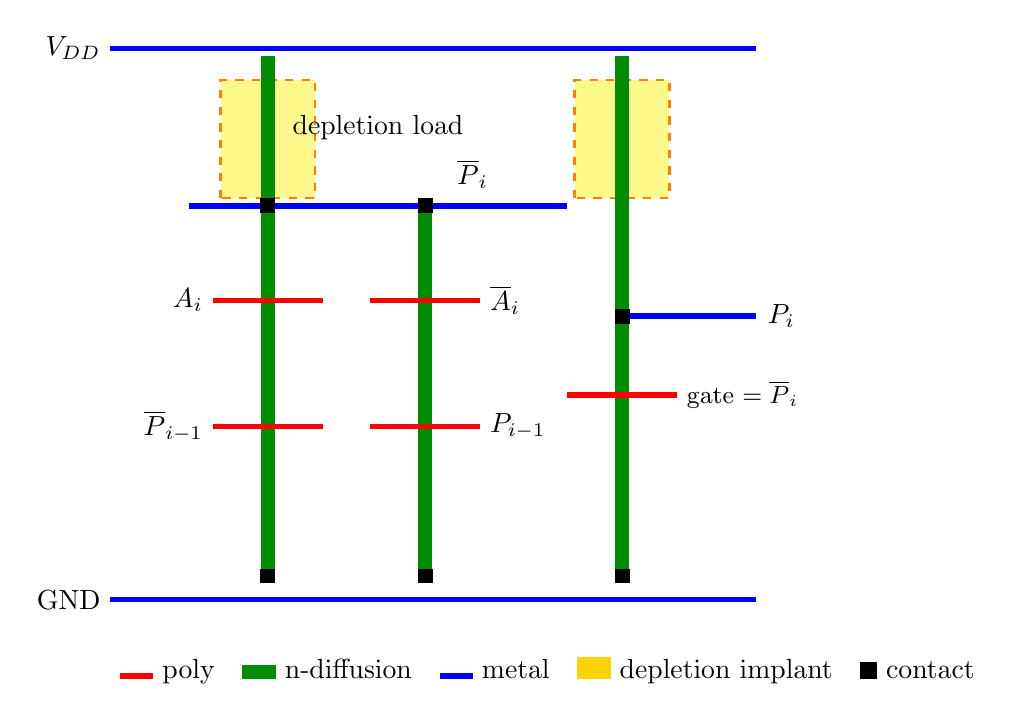
\begin{tikzpicture}[
  poly/.style={red, line width=2pt},
  ndiff/.style={green!55!black, line width=5pt},
  metal/.style={blue, line width=2pt},
  implant/.style={fill=yellow!45, draw=orange, dashed, line width=1pt},
  cont/.style={fill=black, draw=black, minimum size=5pt, inner sep=0pt}]
% rails
\draw[metal] (0,7) -- (8.2,7); \node[left] at (0,7){$V_{DD}$};
\draw[metal] (0,0) -- (8.2,0); \node[left] at (0,0){GND};
% depletion pull-up (left)
\draw[implant] (1.4,5.1) rectangle (2.6,6.6);
\draw[ndiff] (2,6.9) -- (2,5);
\node at (3.4,6.0){depletion load};
% Pbar_i metal node
\draw[metal] (1.0,5) -- (5.0,5); \node[above] at (4.6,5.1){$\overline{P}_i$};
% two pull-down branches
\draw[ndiff] (2,5) -- (2,0.3);
\draw[ndiff] (4,5) -- (4,0.3);
% poly gate lines crossing the branches
\draw[poly] (1.3,3.8) -- (2.7,3.8); \node[left] at (1.3,3.8){$A_i$};
\draw[poly] (1.3,2.2) -- (2.7,2.2); \node[left] at (1.3,2.2){$\overline{P}_{i-1}$};
\draw[poly] (3.3,3.8) -- (4.7,3.8); \node[right] at (4.7,3.8){$\overline{A}_i$};
\draw[poly] (3.3,2.2) -- (4.7,2.2); \node[right] at (4.7,2.2){$P_{i-1}$};
\foreach \x in {2,4}{ \node[cont] at (\x,0.3){}; \node[cont] at (\x,5){}; }
% inverter (right) -> P_i
\draw[implant] (5.9,5.1) rectangle (7.1,6.6);
\draw[ndiff] (6.5,6.9) -- (6.5,0.3);
\draw[metal] (5.0,5) -- (5.8,5);
\draw[poly] (5.8,2.6) -- (7.2,2.6); \node[right] at (7.2,2.6){\small gate $=\overline{P}_i$};
\draw[metal] (6.5,3.6) -- (8.2,3.6) node[right,black]{$P_i$};
\node[cont] at (6.5,0.3){}; \node[cont] at (6.5,3.6){};
% legend
\node[anchor=west, align=left] at (0,-0.9)
 {\textcolor{red}{$\rule{12pt}{2pt}$} poly\quad
  \textcolor{green!55!black}{$\rule{12pt}{5pt}$} n-diffusion\quad
  \textcolor{blue}{$\rule{12pt}{2pt}$} metal\quad
  \textcolor{yellow!70!orange}{$\rule{12pt}{8pt}$} depletion implant\quad
  \rule{6pt}{6pt}~contact};
\end{tikzpicture}
\end{document}
